\documentclass[a4paper, 12pt]{article}
\usepackage{graphicx}
\usepackage[margin=2cm]{geometry}
\usepackage[hidelinks]{hyperref}
\usepackage[croatian]{babel}
\usepackage[sorting=none]{biblatex}
    \addbibresource{ref.bib}
\usepackage{float}


% Boje za kod:
\usepackage{xcolor,graphicx}
\usepackage{listings}

\definecolor{solarized-base03}{RGB}{0, 43, 54}
\definecolor{solarized-base02}{RGB}{7, 54, 66}
\definecolor{solarized-base01}{RGB}{88, 110, 117}
\definecolor{solarized-base00}{RGB}{101, 123, 131}
\definecolor{solarized-base0}{RGB}{131, 148, 150}
\definecolor{solarized-base1}{RGB}{147, 161, 161}
\definecolor{solarized-base2}{RGB}{238, 232, 213}
\definecolor{solarized-base3}{RGB}{253, 246, 227}
\definecolor{solarized-yellow}{RGB}{181, 137, 0}
\definecolor{solarized-orange}{RGB}{203, 75, 22}
\definecolor{solarized-red}{RGB}{220, 50, 47}
\definecolor{solarized-magenta}{RGB}{211, 54, 130}
\definecolor{solarized-violet}{RGB}{108, 113, 196}
\definecolor{solarized-blue}{RGB}{38, 139, 210}
\definecolor{solarized-cyan}{RGB}{42, 161, 198}
\definecolor{solarized-green}{RGB}{133, 153, 0}

\lstset{
  basicstyle=\footnotesize\ttfamily\color{solarized-base00},
  keywordstyle=\color{solarized-blue}\bfseries,
  commentstyle=\color{solarized-base1},
  stringstyle=\color{solarized-cyan},
  identifierstyle=\color{solarized-violet},
  numberstyle=\tiny\color{solarized-base01},
  numbers=left,
  firstnumber=1,
  stepnumber=1,
  showstringspaces=false,
  tabsize=4,
  frame=none,
  framerule=1pt,
  framexleftmargin=5pt,
  framexrightmargin=5pt,
  framextopmargin=3pt,
  framexbottommargin=3pt,
  backgroundcolor=\color{solarized-base3},
  rulecolor=\color{solarized-base01},
  breaklines=true,
  breakatwhitespace=true,
  language=C++
}


\begin{document}
\noindent
Univerzitet u Sarajevu\\
Elektrotehnički fakultet\\
Predmet: Uvod u digitalnu obradu slike\\
Predmetni profesor: prof. dr Emir Sokić\\
Autor: Berina Biberović\\
Akademska godina: 2022/2023.


\begin{center}
    \section*{Tutorijal 10}
    \subsection*{Lokalni deskriptori}
\end{center}

Pitanje na koje želimo odgovoriti ovaj tutorijal je kako objasniti našem programu šta su deskriptori koji opisuju dijelove na slici, na način na koji mi, kao ljudi, to shvatamo. To je veoma teško pitanje, ali potrudit ćemo se da damo uvod u ovu oblast.

Teško je objasniti kako ljudi percipiraju deskriptore unutar naših umova - oni su već "isprogramirani" unutar naših mozgova. Ali, možemo uočiti nešto interesantno ako gledamo dublje u neke slike i tražimo različite šablone. Najbolji primjer za ovo se može naći na \href{https://docs.opencv.org/3.4/df/d54/tutorial_py_features_meaning.html}{linku}. Preporučuje se studentima da pročitaju ovaj kratki uvod o kojem i profesor priča na predavanju.

\subsection*{\textit{SIFT}}

\textit{Scale Invariant Feature Transform} je algoritam koji izdvaja ključne tačke (eng. \textit{keypoints}) i računa njihove deskriptore. \textit{SIFT} algoritam radi u četiri koraka, u čije detalje mi nećemo ulaziti na ovom tutorijalu (ukoliko želite da naučite više o ovom algoritmu, to možete uraditi tako što pročitate informacije na OpenCV stranici na \href{https://docs.opencv.org/3.4/da/df5/tutorial_py_sift_intro.html}{linku}). Mi ćemo na ovom tutorijalu naučiti kako da iskoristimo gotovu implementaciju ovog algoritma u OpenCV-u.

Unutar OpenCV-a postoji klasa \lstinline{cv::SIFT} koju ćemo iskoristiti za implementaciju \textit{SIFT} algoritma. U nastavku slijedi primjer koda koji će biti detaljno objašnjen.

\begin{lstlisting}
#include <opencv4/opencv2/core.hpp>
#include <opencv4/opencv2/imgproc.hpp>
#include <opencv4/opencv2/highgui.hpp>
#include <opencv2/features2d.hpp>
#include <opencv2/calib3d.hpp>
#include <vector>
#include <algorithm>

int main() {

    // Kreiranje pametnog pokazivaca na objekat tipa cv::SIFT:
    cv::Ptr<cv::SIFT> sift = cv::SIFT::create();

    // Ucitavanje slike:
    cv::Mat slika = cv::imread("../Slika1.jpg", cv::IMREAD_GRAYSCALE);
    cv::Mat sablon = cv::imread("../SablonAS.jpg", cv::IMREAD_GRAYSCALE);

    // Pravimo vektore za keypoints na slici i na sablonu:
    std::vector<cv::KeyPoint> keypoints_slika, keypoints_sablon;

    // Pravimo matricu za deskriptore i na slici i na sablonu:
    cv::Mat deskriptori_slika, deskriptori_sablon;

    // Samo pozovemo funkciju za racunanje keypoint-a i deskriptora:
    sift->detectAndCompute(slika, cv::noArray(), keypoints_slika, deskriptori_slika, false);
    sift->detectAndCompute(sablon, cv::noArray(), keypoints_sablon, deskriptori_sablon, false);

    // Sada pozivamo funkciju koja ce da nacrta keypoints na slici i na sablonu:
    cv::Mat pomocna_slika, pomocni_sablon;
    cv::drawKeypoints(slika, keypoints_slika, pomocna_slika, cv::Scalar::all(-1), cv::DrawMatchesFlags::DEFAULT);
    cv::drawKeypoints(sablon, keypoints_sablon, pomocni_sablon, cv::Scalar::all(-1), cv::DrawMatchesFlags::DEFAULT);

    // Prikaz izvadjenih keypoint-a:
    cv::imshow("Keypoints na slici", pomocna_slika);
    cv::imshow("Keypoints na sablonu", pomocni_sablon);
    cv::waitKey();

    return 0;
}
\end{lstlisting}

Prva stvar koju je potrebno uraditi jeste napraviti pametni pokazivač \lstinline{cv::Ptr} na tip \lstinline{cv::SIFT} i onda ga inicijalizirati (tj. kreirati) preko konstrukcije koja je pokazana u liniji 10: \lstinline{cv::SIFT::create()}. Nakon toga na standardni način učitavamo sliku na kojoj želimo pronaći šablon (koji isto tako učitamo na standardan način). Primijetite da se slike učitavaju u \textit{grayscale} obliku.

Potrebno je onda napraviti dva vektora čiji su elementi tipa \lstinline{cv::KeyPoint} - ova klasa unutar OpenCV-a nam omogućava da iskroistimo funkcije za računanje \textit{keypoint}-a. U oba ta vektora će biti upisani odgovarajuće ključne tačke nakon što funkcija za detektovanje obavi svoj posao. Nakon toga nam trebaju dva parametra \lstinline{cv::Mat} tipa, u koje ćemo moći upisati deskriptore obje učitane slike.

U linijama 23 i 24 smo iskoristili funkciju \lstinline{detectAndCompute} koja je funkcija članica \lstinline{cv::Feature2D} klase. Ona prima sljedeće parametre: parametar tipa \lstinline{InputArray} koji predstavlja sliku na kojoj tražimo ključne tačke i deskriptore; parametar tipa \lstinline{InputArray} koji predstavlja masku - u našem slučaju mi smo proslijedili parametar \lstinline{cv::noArray}; parametar tipa \lstinline{std::vector<cv::Keypoint>&} koji predstavlja vektor u koji se upisuju ključne tačke; parametar tipa \lstinline{OutputArray} u koji se upisuju pronađeni deskriptori; parametar tipa \lstinline{bool} koji je preklopljen i postavljen na \lstinline{false}, osim ako mu se ne proslijedi \lstinline{true}.

Prikazani kod je uspješno izračunao \textit{keypoints} i deskriptore na slici na kojoj tražimo odgovarajući šablon. Rezultate ćemo pokaziti na pomoćnim slikama preko funkcije \lstinline{cv::drawKeypoints} koja prima: parametar \lstinline{InputArray} koji je zapravo ulazna slika na kojoj smo našli ključne tačke prethodnom funkcijom; parametar tipa \lstinline{const std::vector<cv::Keypoint>&} koji predstavlja pronađene ključne tačke; parametar tipa \lstinline{InputOutputArray} koji je izlazna slika ove funkcije na koju će se nacrtati ključne tačke; parametar tipa \lstinline{const Scalar &} koji predstavlja boju nacrtanih ključnih tačaka i preklopljen je na \lstinline{cv::Scalar::all(-1)}; parametar tipa \lstinline{int} koji predstavlja \textit{flag} koji su tipa \lstinline{anonymous enum} i preklopljen je na \lstinline{cv::DrawMatchesFlags::DEFAULT}.

Na slici \ref{sl1} imamo prikazanu izvornu ulaznu sliku, dok na slici \ref{sl2} imamo prikazane nacrtane ključne tačke na ulaznoj slici. Slično na slici \ref{sl3} je prikazan originalni šablon koji ćemo tražiti na ulaznoj slici, dok su na slici \ref{sl4} prikazane ključne tačke sa šablona.

\begin{figure}[H]
    \minipage{0.49\textwidth}
        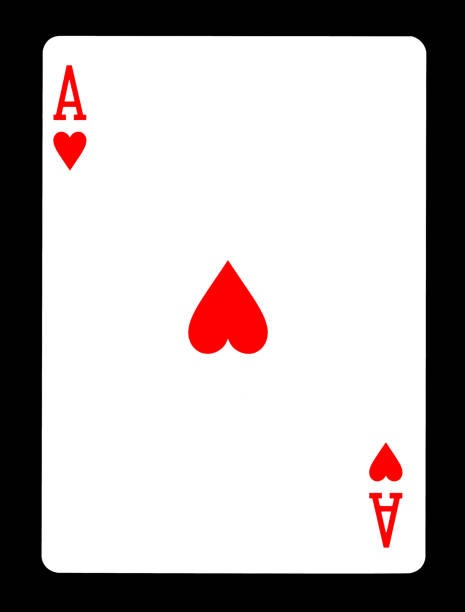
\includegraphics[width=\linewidth]{Slike/Slika1.jpg}
        \caption{Ulazna originalna slika karte (\textit{non-grayscale})}\label{sl1}
    \endminipage\hfill
    \minipage{0.49\textwidth}
        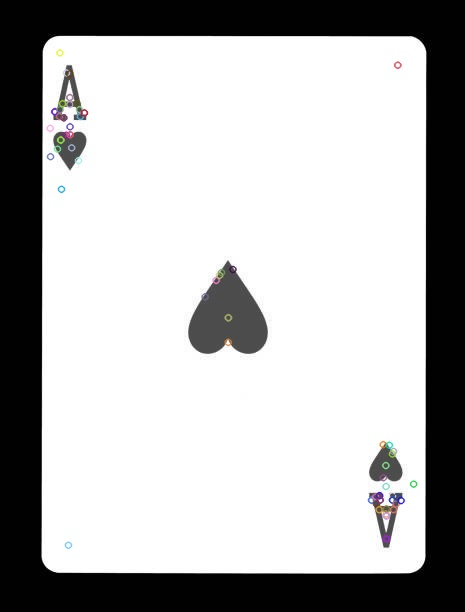
\includegraphics[width=\linewidth]{Slike/slika_rez_keypoints.jpg}
        \caption{Nacrtane ključne tačke na ulaznoj slici (\textit{grayscale})}\label{sl2}
    \endminipage\hfill
\end{figure}

\begin{figure}[H]
\begin{center}
    \minipage{0.4\textwidth}
        
\includegraphics[width=2cm]{Slike/SablonAS.jpg}
        \caption{Originalna šablon slika}\label{sl3}
    \endminipage
    \minipage{0.4\textwidth}
        
\includegraphics[width=2cm]{Slike/sablon_rez_keypoints.jpg}
        \caption{Ključne tačke na šablonu}\label{sl4}
    \endminipage
\end{center}
\end{figure}

Nakon što smo pronašli sve ključne tačke i sve deskriptore, potrebno je da vidimo koje ključne tačke se podudaraju na ulaznoj slici i na šablonu. Kod kako ćemo taj problem riješiti je prikazan u nastavku.

\begin{lstlisting}
    // Potrebno je naci koji deskriptori se podudaraju za ulaznu sliku i za sablon:
    cv::BFMatcher matcher(cv::NORM_L2);
    std::vector<cv::DMatch> matches;

    matcher.BFMatcher::match(deskriptori_sablon, deskriptori_slika, matches);

    // Sada gledamo koliko su koji matchevi "udaljeni":
    double max_udaljenost;
    std::vector<double> udaljenosti;

    for(int i  = 0; i < matches.size(); i++)
        udaljenosti.push_back(matches.at(i).distance);

    // Pronadjemo najvecu udaljenost dva matcha:
    max_udaljenost = *std::max_element(udaljenosti.begin(), udaljenosti.end());

    // Postavimo threshold za matcheve na osnovu max_udaljenost:
    double k = 0.1;
    double threshold = k * max_udaljenost;

    // Sada upisujemo sve matcheve koji su ispod thresholda u novi vektor za podudaranja:
    std::vector<cv::DMatch> podudaranja;

    for(int i = 0; i < matches.size(); i++)
        if(udaljenosti.at(i) <= threshold)
            podudaranja.push_back(matches.at(i));

    // Na kraju crtamo sva podudaranja koju su bila ispod gore navedenog thresholda:
    cv::Mat pomocna_slika2;
    cv::drawMatches(sablon, keypoints_sablon, slika, keypoints_slika, podudaranja, pomocna_slika2, cv::Scalar::all(-1), cv::Scalar::all(-1), std::vector<char>(), cv::DrawMatchesFlags::DEFAULT);

    cv::imshow("Rezultat", pomocna_slika2);
    cv::waitKey();
\end{lstlisting}

Koristimo instancu klase \lstinline{cv::BFMatcher} (\textit{Brute-force matcher}) koju incijaliziramo preko preklopljenog konstruktora sa \lstinline{enum} tipom \lstinline{cv::NORM_L2}. Nakon toga napravimo vektor sa elemntima tipa \lstinline{cv::DMatch} klase.

Koristimo funkciju članicu \lstinline{match} iz klase \lstinline{cv::BFMatcher} kako bismo pronašli koji deskriptori između ulazne slike i šablona se podudaraju. Za što bolje rezultate, potrebno je da suzimo opseg podudaranja. Za to smo iskoristili linije od 7 do 19. Nakon što smo izračunali vrijednost varijable \lstinline{threshold}, onda u novi vektor elemenata \lstinline{cv::DMatch} upisujemo sva podudaranja koja su manja ili jednaka vrijednosti varijable \lstinline{threshold}. 

Na kraju svega pozivamo funkciju \lstinline{cv::drawMatches} koja prima sljedeće parametre: parametar tipa \lstinline{InputArray} koji je prva slika za koju tražimo podudaranje; parametar tipa \lstinline{const std::vector<cv::Keypoint>&} koji predstavlja ključne tačke za prvu sliku; treći i četvrti parametar su isti kao prvi i drugi, samo što se odnose na drugu sliku; peti parametar je tipa \lstinline{const std::vector<cv::DMatch>} koji predstavlja podudaranja koja smo izdvojili prethodno; šesti parametar je slika u koju ćemo upisati rezultate podudaranja; posljednja četiri parametra su \textit{overloaded}/preklopljena, ali navedene su njihove \lstinline{default} vrijednosti unutar koda.

Rezultat koji smo dobili je prikazan na slici \ref{sl5}. Vidimo da smo na ovaj način dobili podudaranja između šablona i ulazne slike, a i pored toga smo smanjili relevantna podudaranja sa gore prikazanim kodom.

\begin{figure}[H]
    \centering
    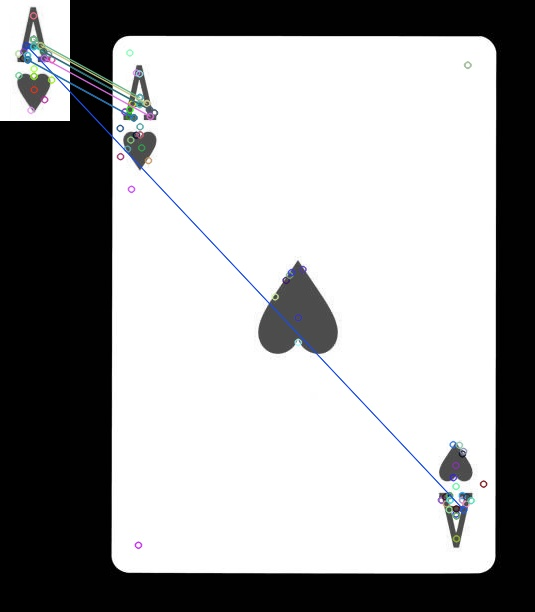
\includegraphics[width=\textwidth]{Slike/konacni.jpg}
    \caption{Konačni rezultat nakon \textit{Brute-force matcher}-a}
    \label{sl5}
\end{figure}

\subsection*{ORB}

\textit{Oriented FAST and Rotated BRIEF} algoritam je napravljen u sklopu OpenCV-a. Ono što nije rečeno za \textit{SIFT} i njegov brži algoritam \textit{SURF} (koji nije spomenut do sada u tutorijalu, ali jeste rađen na predavanju) je to da su ova dva algoritma patentirana. Ako želite da ih koristite u nekoj svojoj komercijalnoj aplikaciji, morat ćete da platite licencu za korištenje. \textit{ORB} nema takvih problema jer je \textit{open source}. 

\textit{ORB} algoritam je efikasna alternativa \textit{SIFT}-u i \textit{SURF}-u u komuptacijskoj cijeni, a performansa je dovoljno dobra. Ovaj algoritam je fuzija \textit{FAST keypoint} detektora i \textit{BRIEF} deskriptora sa mnogo modifikacija kako bi imao što bolje performanse. Detalje o ovom algoritmu možete naći na \href{https://docs.opencv.org/3.4/d1/d89/tutorial_py_orb.html}{linku}.

Ono što nas zanima za primjene ovog tutorijala je kako da primijenimo ovaj algoritam. Odgovor je jednostavan. Samo je potrebno da promijenimo 12. liniju prvog koda sa ovog tutorijala i odgovarajuće varijable i to je to!

\begin{lstlisting}
    cv::Ptr<cv::Feature2D> orb = cv::ORB::create();
\end{lstlisting}

Nemojte zaboraviti da napravite izmjene i u linijama 25 i 26 gdje sada umjesto \lstinline{sift->} treba da piše \lstinline{orb->}. Vjerovatno ćete isto trebati promijeniti vrijednost parametara \lstinline{k} i \lstinline{threshold}, kako bi što bolje radio detektor ključnih tačaka.

\subsection*{Zadatak 1}

Izmijeniti prvi primjer sa \textit{SIFT} algoritmom u \textit{ORB} algoritam i komentarišite razlike koje ste dobili.

\subsection*{Napomene}

Korištena tema za prikaz C++ koda na tutorijalima je \href{https://ethanschoonover.com/solarized/}{\lstinline{solarized}}\cite{solarized}.

\printbibliography


\end{document}